% =====================================================================================
\section{Device and finite-element models}
\label{sec:models}
% =====================================================================================

\subsection{The device}
\label{sec:device}

One silicon-on-insulator design is used throughout (\cref{tab:device}). TE-polarised light at
\qty{1550}{\nano\metre} is split equally into \num{33} strip waveguides at \qty{2}{\micro\metre} pitch, which cross a
heated section about \qty{1}{\milli\metre} long and then reach the grating emitters. The heaters sit before the
gratings, not over them, so the gratings stay at a uniform temperature, the heater length is free, and a vertical
bow of the heated section adds no phase to the emitted light.

\begin{table}[htbp]
  \centering
  \caption{Device parameters. $x$ is across the array; $y=0$ is the top of the buried oxide.}
  \label{tab:device}
  \small
  \begin{tabular}{@{}lp{0.33\linewidth}p{0.34\linewidth}@{}}
    \toprule
    Item & Value & Note \\
    \midrule
    Waveguide core & $\qty{500}{\nano\metre}\times\qty{220}{\nano\metre}$ silicon & in silica \\
    Array & $N=33$, $d=\qty{2}{\micro\metre}$ & emitters at $x=0,\pm2,\dots,\pm\qty{32}{\micro\metre}$ \\
    Buried oxide; top cladding & \qty{2}{\micro\metre}; \qty{2}{\micro\metre} above the core & \\
    Heater & TiN, $\qty{2}{\micro\metre}\times\qty{120}{\nano\metre}$ & \qty{2}{\micro\metre} above the core;
        $\Lh=\qty{1}{\milli\metre}$ where a temperature is quoted \\
    Substrate & silicon, bottom at \qty{293.15}{\kelvin} & \qty{100}{\micro\metre} simulated \\
    Undercut cavity & \qty{80}{\micro\metre} wide, \qty{15}{\micro\metre} deep & walls at $x=\pm\qty{40}{\micro\metre}$ \\
    Slot & \qty{2}{\micro\metre} wide at $x=\qtyrange{36}{38}{\micro\metre}$ & through the whole membrane \\
    Grating & \qty{20}{\nano\metre} teeth, \qty{0.69}{\micro\metre} period & emits at \ang{9.64} in air \\
    \bottomrule
  \end{tabular}
\end{table}

Four thermal structures are compared (\cref{fig:stacks}). They share every dimension and differ only in where the
heat can leave:
\begin{description}[leftmargin=1.6em,itemsep=1pt]
  \item[\stack{Standard}:] solid substrate \qty{2}{\micro\metre} below the cores; the conventional stack.
  \item[\stack{Undercut}:] substrate removed under the array, leaving a \qty{4.2}{\micro\metre} oxide membrane
        anchored to the cavity walls.
  \item[\stack{Slot}:] the undercut with a slot through the membrane just past the edge heater, in air.
  \item[\stack{Vacuum}:] the slot design with no gas in the cavity or the slot.
\end{description}

\begin{figure}[htbp]
  \centering
  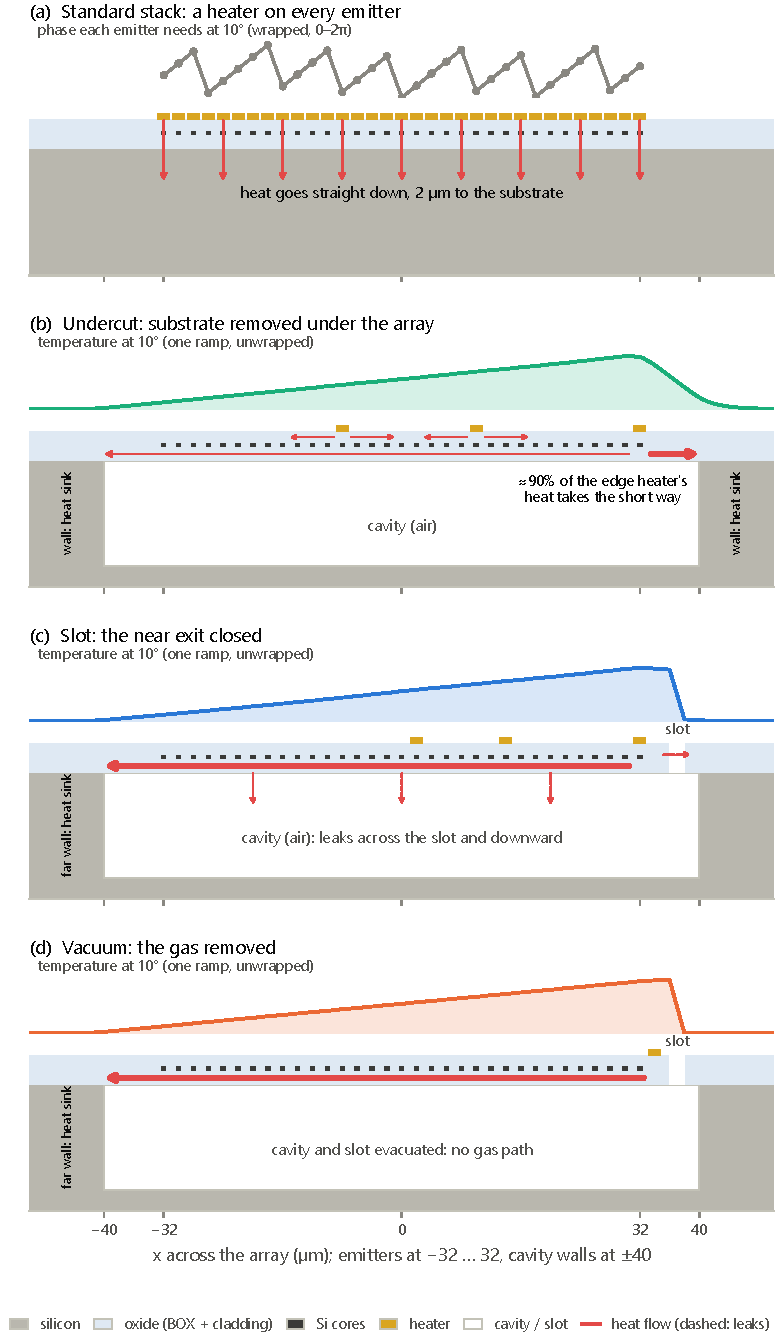
\includegraphics[height=0.62\textheight,width=\linewidth,keepaspectratio]{fig01_stacks}
  \caption{The four structures (cross-sections; heater and core thickness exaggerated), each with the phase
  profile it makes at \ang{10}. (a)~\stack{Standard}: heat flows straight into the substrate, so each emitter needs
  its own heater with a wrapped phase. (b)~\stack{Undercut}: heat spreads sideways to both cavity walls, but the
  edge heater loses most of its heat to the nearby wall. (c)~\stack{Slot}: the slot closes that short path, so the
  heat crosses the array and the temperature falls as a ramp; air still conducts some heat across the slot and into
  the cavity. (d)~\stack{Vacuum}: with no gas, the far wall is the only heat sink.}
  \label{fig:stacks}
\end{figure}

\subsection{Finite-element models}

Three two-dimensional models, built in COMSOL Multiphysics~6.3~\cite{comsol}, supply every physical input
(\cref{tab:models}). Each exports tables that the Python analysis reads directly. Meshes are free triangular, with elements of
\qtyrange{25}{35}{\nano\metre} in the cores and heater and \qtyrange{130}{250}{\nano\metre} in the oxide; their
adequacy is checked in \cref{sec:comsolchecks}.

\begin{table}[htbp]
  \centering
  \caption{The three finite-element models and their studies.}
  \label{tab:models}
  \small
  \begin{tabularx}{\linewidth}{@{}P{0.13\linewidth}P{0.4\linewidth}L@{}}
    \toprule
    Model & Studies & Outputs used \\
    \midrule
    Waveguide & mode analysis of one strip, swept in temperature and wavelength; even and odd supermodes of a
        pair, swept in spacing & $\neff$, $\dndT$, element pattern, group index; coupling length \\
    Thermal & stationary heat transfer with one heater swept across the array, for each structure; coupled
        heat-and-mode solve; step responses; temperature-dependent conductivity with two heaters & kernels
        $R(x;\xh)$; check of \cref{eq:phaseT}; transients; limits of linearity and superposition \\
    Grating & frequency-domain side view of one grating with ports and absorbing layers & emission angle and its
        rates with period, wavelength and temperature; leakage length \\
    \bottomrule
  \end{tabularx}
\end{table}

\subsubsection{Waveguide model}
\label{sec:modelA}

A mode solve of one core in a \qty{4}{\micro\metre} silica box ($n_\mathrm{Si}=3.476$, $n_\mathrm{SiO_2}=1.444$,
thermo-optic coefficients \qty{1.86e-4}{} and \qty{0.95e-5}{\per\kelvin}) gives $\neff=\num{2.44546}$. A uniform
temperature sweep over \qty{100}{\kelvin} gives
\begin{equation}
  \frac{\dd\neff}{\dd T} \;=\; \qty{2.009e-4}{\per\kelvin},
\end{equation}
linear to \num{3.5e-6} and \num{1.08} times the bulk value, because the mode is concentrated in the core
(\cref{fig:mode}). The element pattern is taken as the Fourier transform of the mode's $E_x$ summed over height; it
is \num{0.90} at \ang{20} and \num{0.87} at \ang{22.8}, and changes by less than \qty{1}{\percent} over
\qty{100}{\kelvin}. A wavelength sweep gives the group index, $n_g=4.18$.

The same model, reduced to a half-model with a perfect electric or magnetic conductor on the mirror plane, gives the
even and odd supermodes of two waveguides. Solving both on one mesh cancels the discretisation error in their
index difference $\Delta n$, which falls exponentially with spacing. The coupling length $L_c=\lambda/(2\Delta n)$
is \qty{2.2}{\metre} at \qty{2}{\micro\metre} pitch, and under \qty{1}{\percent} of the power transfers over
\qty{2}{\milli\metre} for any pitch above \qty{1.5}{\micro\metre}. Optical coupling is therefore
neglected.

\begin{figure}[htbp]
  \centering
  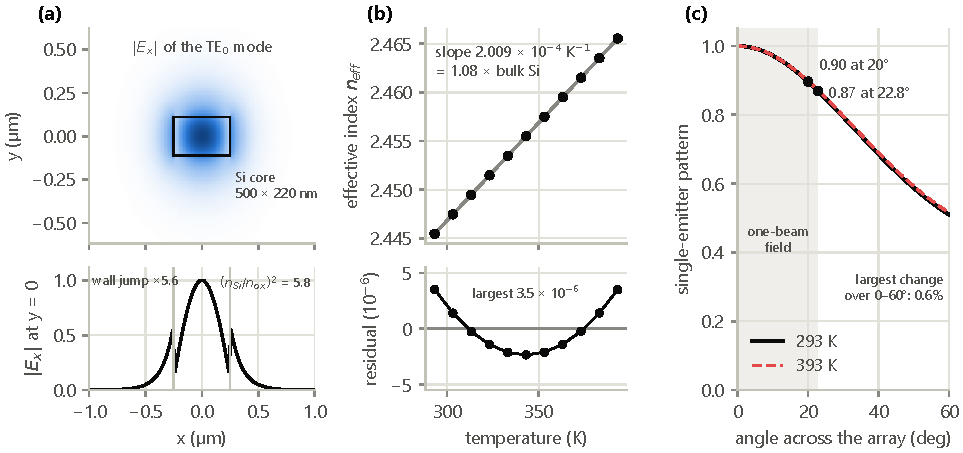
\includegraphics[width=\linewidth]{rep_mode}
  \caption{Waveguide model. (a)~$|E_x|$ of the TE mode, with a cut through the core centre; the field jumps at the
  side walls as continuity of the normal displacement requires. (b)~Effective index against temperature with its
  linear fit. (c)~Element pattern at \qty{293}{\kelvin} and \qty{393}{\kelvin}.}
  \label{fig:mode}
\end{figure}

\subsubsection{Thermal model}
\label{sec:modelC}\label{sec:modelF}

One cross-section model provides all thermal results. It contains a \qty{300}{\micro\metre}-wide,
\qty{100}{\micro\metre}-deep silicon substrate, the buried oxide, \num{33} silicon cores, the cladding and a TiN
heater that can be placed anywhere, dissipating \qty{1}{\watt\per\metre}. The substrate bottom is held at ambient
and all other boundaries are insulated; convection from the top surface would remove under \qty{1}{\percent} of
the heat. Conductivities are \qty{148}{} (Si), \qty{1.38}{} (SiO$_2$), \qty{25}{} (TiN) and
\qty{0.026}{\watt\per\metre\per\kelvin} (air). Parameters switch the structure: a cavity region becomes silicon
(\stack{standard}) or air (\stack{undercut}); a slot region through the membrane becomes oxide or air
(\stack{slot}); the gas conductivity becomes \qty{e-4}{\watt\per\metre\per\kelvin} (\stack{vacuum}; this value also
bounds black-body radiation across the cavity, $4\sigma T^3D\approx\qty{0.9e-4}{\watt\per\metre\per\kelvin}$). Four
studies were run:

\begin{enumerate}
  \item \emph{Kernels.} The temperature rise along the line through the cores, for heater positions swept in
        \qty{1}{} or \qty{2}{\micro\metre} steps: one solve for the \stack{standard} stack, whose kernel depends only
        on $x-\xh$; $\xh=0$ to \qty{40}{\micro\metre} for the \stack{undercut} (mirrored for negative positions);
        $-32$ to \qty{34}{\micro\metre} for the \stack{slot} and \stack{vacuum}, which have no mirror symmetry.
        Six further solves test the stack (\cref{sec:comsolchecks}).
  \item \emph{Coupled heat and mode.} A mode solve inside the temperature field of a heater 0, 2 and
        \qty{4}{\micro\metre} from a core, to test \cref{eq:phaseT} in a non-uniform field.
  \item \emph{Step responses.} The time-dependent response to switching a heater on, at all \num{33} cores, for
        each structure, to \qty{32}{\milli\second}.
  \item \emph{Nonlinearity.} Conductivities made temperature-dependent ($k_\mathrm{Si}\propto T^{-1.3}$,
        $k_\mathrm{SiO_2}\propto1+\qty{8e-4}{\per\kelvin}\,\Delta T$), with heater powers raised until the core is
        about \qty{185}{\kelvin} above ambient, and a second heater \qty{6}{\micro\metre} away for the superposition
        test of \cref{sec:superposition}.
\end{enumerate}

\subsubsection{Grating model}
\label{sec:modelE}

A side view of one grating gives the behaviour along the waveguides. Because the strip is three-dimensional, the
two-dimensional model uses an equivalent core of index \num{3.0604} that reproduces the strip's $\neff$ and
$\dndT$ exactly; emission angles and their rates with period and temperature therefore carry over to the real
waveguide. The rate with wavelength is corrected using the strip's group index, and the emission strength is
approximate. The model is excited through a port and terminated by absorbing layers; \num{18} runs vary period,
wavelength and temperature (results in \cref{sec:gratingaxis}).
